\documentclass{beamer}

\usepackage{kotex}
\usepackage{graphicx,psfrag,amsfonts,amsmath,amssymb}
\usepackage{multicol}
\usepackage{algorithm2e}

\usetheme{metropolis}
\usefonttheme[onlymath]{serif}	% 수식 설정!!
\setbeamertemplate{section in toc}[sections numbered]

\title{PC Selection for Sparse FPCA}
%\date{\today}
\date[Short Occasion]{October 1, 2019}
\author{Hyunsung Kim}
\institute{Department of Statistics\\ Chung-Ang University}

% A subtitle is optional and this may be deleted
\subtitle{}

%\author{F.~Author\inst{1} \and S.~Another\inst{2}}
% - Give the names in the same order as the appear in the paper.
% - Use the \inst{?} command only if the authors have different
%   affiliation.

%\institute[Universities of Somewhere and Elsewhere] % (optional, but mostly needed)
%{
%  \inst{1}%
%  Department of Computer Science\\
%  University of Somewhere
%  \and
%  \inst{2}%
%  Department of Theoretical Philosophy\\
%  University of Elsewhere}
% - Use the \inst command only if there are several affiliations.
% - Keep it simple, no one is interested in your street address.

%\date{Conference Name, 2013}
% - Either use conference name or its abbreviation.
% - Not really informative to the audience, more for people (including
%   yourself) who are reading the slides online

\subject{Functional Data Analysis}
% This is only inserted into the PDF information catalog. Can be left
% out. 

% If you have a file called "university-logo-filename.xxx", where xxx
% is a graphic format that can be processed by latex or pdflatex,
% resp., then you can add a logo as follows:

% \pgfdeclareimage[height=0.5cm]{university-logo}{university-logo-filename}
% \logo{\pgfuseimage{university-logo}}

% Delete this, if you do not want the table of contents to pop up at
% the beginning of each subsection:
\AtBeginSubsection[]
{
  \begin{frame}<beamer>{Outline}
    \tableofcontents[currentsection,currentsubsection]
  \end{frame}
}

\def \bY {\mathbf{Y}}
\def \by {\mathbf{y}}
\def \bX {\mathbf{X}}
\def \bB {\mathbf{B}}
\def \bD {\mathbf{D}}
\def \bbeta {\boldsymbol{\beta}}
\def \btheta {\boldsymbol{\theta}}
\def \bTheta {\boldsymbol{\Theta}}
\def \bepsilon {\boldsymbol{\epsilon}}
\def \balpha {\boldsymbol{\alpha}}
\def \bgamma {\boldsymbol{\gamma}}
\def \bGamma {\boldsymbol{\Gamma}}
\def \bR {\boldsymbol{R}}
\def \bZ {\boldsymbol{Z}}
\def \bG {\boldsymbol{G}}
\def \bu {\boldsymbol{u}}
\def \bV {\boldsymbol{V}}


% Let's get started
\begin{document}

\begin{frame}
  \titlepage
\end{frame}

\begin{frame}{Outline}
  \tableofcontents
  % You might wish to add the option [pausesections]
\end{frame}

% Section and subsections will appear in the presentation overview
% and table of contents.
\section{Methods to Choose the Number of PCs}
\begin{frame}{PVE}
	\begin{block}{PVE(Proportion of Variance Explained)}
		\vspace{0.2cm}
%		$$ PVE_i = \frac{\lambda_i}{\sum_{j=1}^{\infty}\lambda_j} $$
%		$$ Cumulative \ PVE = \frac{\sum_{j=1}^{K}\lambda_j}{\sum_{j=1}^{\infty}\lambda_j} $$
		$$ \begin{aligned}
			PVE_i &= \frac{\lambda_i}{\sum_{j=1}^{\infty}\lambda_j} \\
			PVE &= \frac{\sum_{j=1}^{K}\lambda_j}{\sum_{j=1}^{\infty}\lambda_j}
		\end{aligned}
		$$
		
		Select $K$, the number of PCs, where 
%		\vspace{-0.1cm}
		$$ PVE \ge 0.95 $$
%		\begin{itemize}
%			\item {
%				Select $K$, the number of PCs where 
%				\vspace{-0.1cm}
%				$$ Cumulative \ PVE > 0.95 $$
%			}
%			\item {
%				Using the \texttt{EM} option, it solves the reduced rank model(James \textit{et al.}) to obtain FPC functions.
%			}		
%			\item {
%				It uses PACE method(Yao \textit{et al.}) not the numerical integration to estimate FPC scores.
%			}
%		\end{itemize}
	\end{block}
\end{frame}


%\section{Cross-Validation}
\begin{frame}{Cross-Validation}
	\begin{block}{Leave-one-curve-out cross validation}
		\vspace{0.1cm}
		$$ LOOCV_i(K) = \frac{1}{N} \sum_{i=1}^N \lVert \bY_i - \widehat{\bY}_i^{-i} \lVert^2  $$
		where
		$$ \widehat{Y_i}^{-i}(t) = \hat\mu(t) + \sum_{k=1}^K \hat\phi_k^{-i}(t) \hat\xi_{ik}^{-i} $$
		
		Select $K$, the number of FPCs, by minimizing the $LOOCV$ score.
	\end{block}
\end{frame}

\begin{frame}{LOOCV with Squared Loss}
	\begin{figure}[h] %%% t: top, b: bottom, h: here
		\begin{center}
			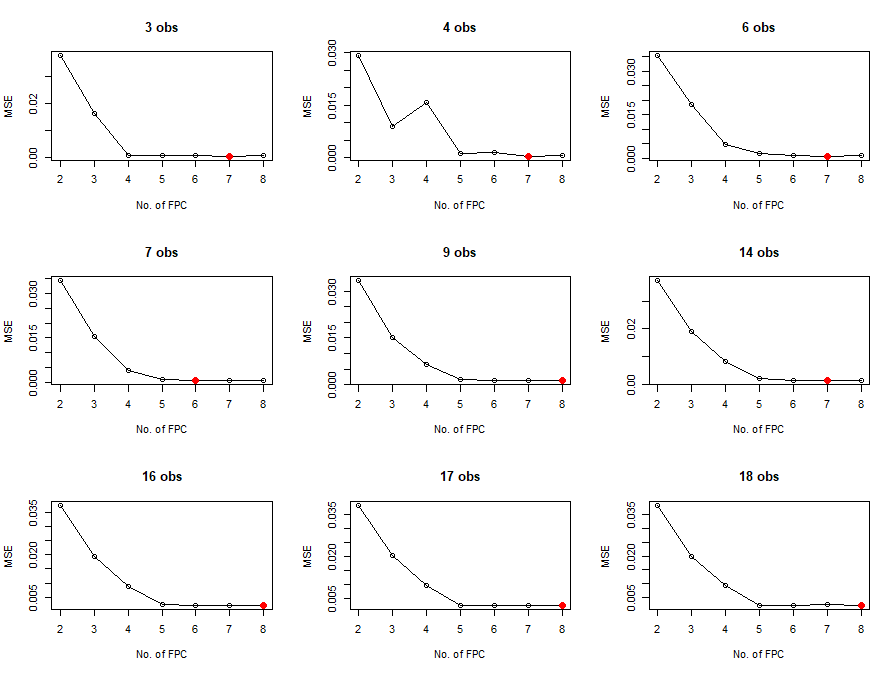
\includegraphics[width=0.8\linewidth]{img/1.png}
		\end{center}
		\label{fig:long}
		\label{fig:onecol}
		\caption{Estimated MSE for 1st training data}
	\end{figure}
\end{frame}

\begin{frame}{LOOCV with Kullback–Leibler Loss(Peng and Paul, 2009)}
	\begin{figure}[h] %%% t: top, b: bottom, h: here
		\begin{center}
			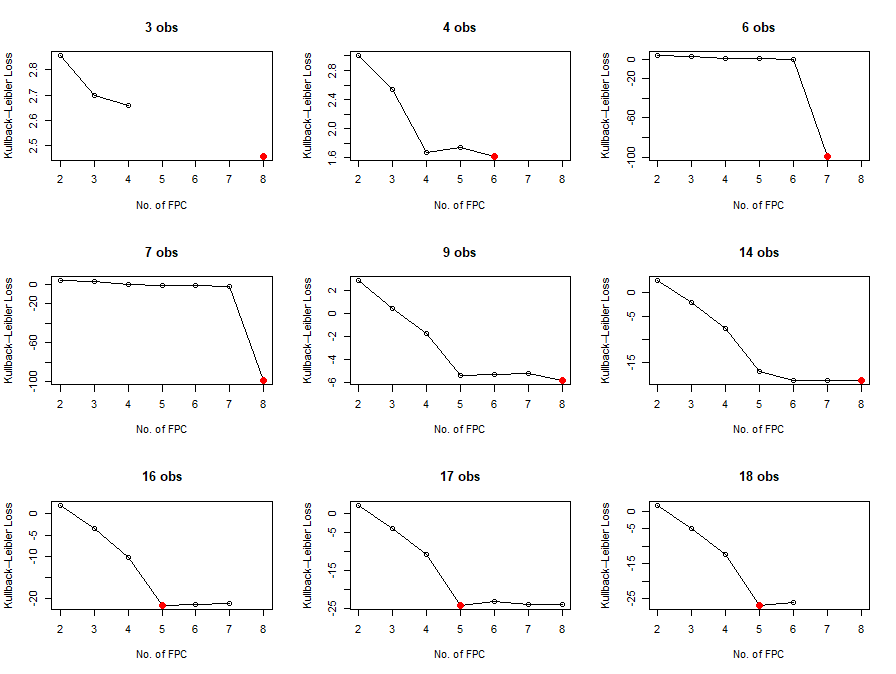
\includegraphics[width=0.8\linewidth]{img/2.png}
		\end{center}
		\label{fig:long}
		\label{fig:onecol}
		\caption{Estimated Kullback–Leibler divergence for 1st training data}
	\end{figure}
\end{frame}


\section{Simulation}
\begin{frame}{Simulation}
	\begin{block}{The Procedure of the Simulation}
		\vspace{0.1cm}
		\begin{itemize}
			\item {
				Generate the $100$ datasets from the temporal gene expression data and 
				split the each dataset with training and test set.
			}
			\item {
				"Sparsify" the each dataset.
			}		
			\item {
				Estimate the FPC functions and scores using the sparse FPCA method with $7$ knots.
			}
			\item {
				Perform the $5$ classification methods for the training sets, and predict for the test sets with the different number of FPCs.
			}
			\item {
				Choose the number of FPCs satisfied $PVE \ge 0.95$
			}
		\end{itemize}
	\end{block}
\end{frame}



\begin{frame}{Simulation Results}
	\begin{table}[ht]
		\caption{Accuracy using FPCs selected by PVE}
		\centering
		\tiny
		\begin{tabular}{cccccccc}
			\hline
			No. \\of obs & Logistic & SVM(Linear) & SVM(Gaussian) & SVM(Sigmoid) & SVM(Poly) & K & PVE \\ 
			\hline
			2 & 0.645 & 0.653 & 0.623 & 0.622 & 0.607 & 3.16 & 0.92 \\ 
			3 & 0.783 & 0.784 & 0.745 & 0.751 & 0.739 & 3.78 & 0.94 \\ 
			4 & 0.848 & 0.846 & 0.800 & 0.834 & 0.803 & 4.15 & 0.97 \\ 
			5 & 0.899 & 0.898 & 0.857 & 0.883 & 0.856 & 4.62 & 0.98 \\ 
			6 & 0.894 & 0.895 & 0.854 & 0.879 & 0.859 & 4.97 & 0.99 \\ 
			7 & 0.915 & 0.913 & 0.879 & 0.899 & 0.879 & 4.99 & 0.99 \\ 
			8 & 0.910 & 0.912 & 0.876 & 0.893 & 0.885 & 5.03 & 0.99 \\ 
			9 & 0.916 & 0.917 & 0.880 & 0.905 & 0.894 & 5.03 & 0.99 \\ 
			10 & 0.917 & 0.919 & 0.884 & 0.904 & 0.886 & 5.00 & 0.99 \\ 
			11 & 0.922 & 0.923 & 0.887 & 0.909 & 0.892 & 5.00 & 0.99 \\ 
			12 & 0.921 & 0.925 & 0.889 & 0.906 & 0.891 & 5.00 & 0.99 \\ 
			13 & 0.919 & 0.921 & 0.888 & 0.908 & 0.892 & 5.00 & 0.99 \\ 
			14 & 0.922 & 0.924 & 0.891 & 0.908 & 0.892 & 5.00 & 0.99 \\ 
			15 & 0.921 & 0.923 & 0.886 & 0.906 & 0.894 & 5.00 & 0.99 \\ 
			16& 0.923 & 0.923 & 0.889 & 0.906 & 0.894 & 5.00 & 0.99 \\ 
			17 & 0.922 & 0.924 & 0.888 & 0.905 & 0.888 & 5.00 & 0.99 \\ 
			18 & 0.923 & \textcolor{red}{0.926} & 0.891 & 0.908 & 0.893 & 5.00 & 0.99 \\ 
			\hline
			Average & 0.888 & \textcolor{red}{0.890} & 0.853 & 0.872 & 0.855 & 4.75 & 0.98 \\
			\hline
		\end{tabular}
	\end{table}
\end{frame}

\begin{frame}{Summary of Results}
	\begin{itemize}
		\item {
			Using PVE, almost $5$ FPCs are selected.
		}	
		\item {
			The selected FPCs explained about 99\% of total variability except $ N_i \le 5 $.
		}	
		\item {
			The linear SVM perform well than other kernel SVM methods.
		}
		\item {
			If there are about $7$ out of $18$ observations, the model answered more than 90\% correctly.
		}
	\end{itemize}
\end{frame}

\begin{frame}{Conclusion}
	\begin{itemize}
		\item {
			LOOCV with squared loss doesn't look like the reliable method.
		}	
		\item {
			Also, LOOCV's computation time is very slow, even though used parallel computing.
		}	
		\item {
			LOOCV with Kullback–Leibler loss looks a better measure than squared loss, but \texttt{fpca.mle} function in \texttt{fpca} package is very unstable.
		}
		\item {
			PVE is the more useful method than LOOCV with squared loss in terms of dimension reduction.
		}
	\end{itemize}
\end{frame}


\appendix
\section{Reference}
\begin{frame}
  \frametitle<presentation>{Reference}
    
  \begin{thebibliography}{10}
  	\beamertemplatearticlebibitems
  	\bibitem{Someone2009}
  	Peng, J. and Paul, D.
  	\newblock A Geometric Approach to Maximum Likelihood Estimation of the Functional Principal Components From Sparse Longitudinal Data
  	\newblock {\em Journal of Computational and Graphical Statistics}, 18(4):995--1015,
  	2009.
		
   	\beamertemplatearticlebibitems
	\bibitem{Someone2005}
		Yao, F. \textit{et al.}
		\newblock Functional data analysis for sparse longitudinal data
		\newblock {\em Journal of the American Statistical Association}, 100(470):577--590,
		2005.
  \end{thebibliography}
\end{frame}


% All of the following is optional and typically not needed. 
%\appendix
%\section<presentation>*{\appendixname}
%\subsection<presentation>*{For Further Reading}
%
%\begin{frame}[allowframebreaks]
%  \frametitle<presentation>{For Further Reading}
%    
%  \begin{thebibliography}{10}
%    
%  \beamertemplatebookbibitems
%  % Start with overview books.
%
%  \bibitem{Author1990}
%    A.~Author.
%    \newblock {\em Handbook of Everything}.
%    \newblock Some Press, 1990.
% 
%    
%  \beamertemplatearticlebibitems
%  % Followed by interesting articles. Keep the list short. 
%
%  \bibitem{Someone2000}
%    S.~Someone.
%    \newblock On this and that.
%    \newblock {\em Journal of This and That}, 2(1):50--100,
%    2000.
%  \end{thebibliography}
%\end{frame}

\end{document}


